(MOS Results, Plots and stuff)

Pure result numbers here only, analysis in evaluation

\textbf{Compare preset MOS}

\begin{figure*}[t!]
	\centering
	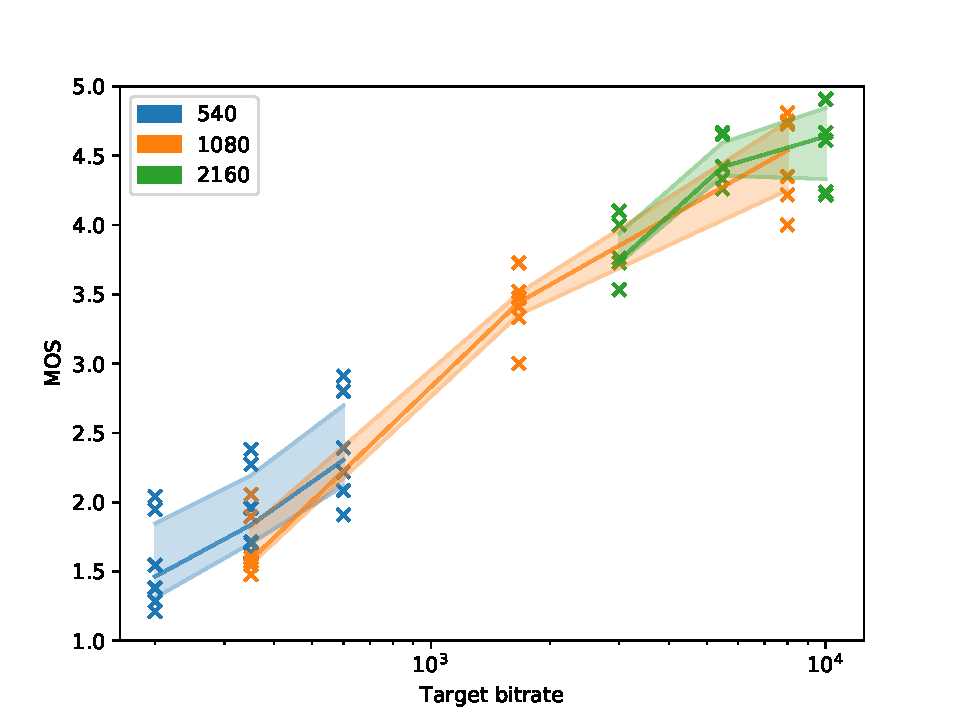
\includegraphics[width=3.5in]{correlation_bitrate_mos_p1}
	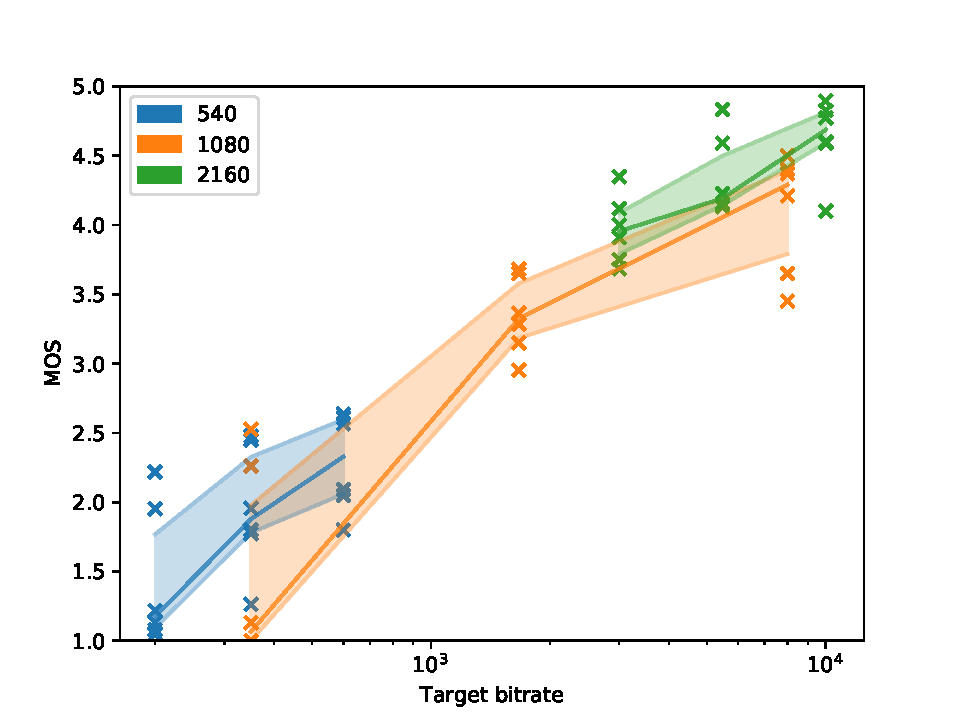
\includegraphics[width=3.5in]{correlation_bitrate_mos_p2}
	\caption{Correlation between bitrate and MOS for both encoding presets. The center line represents a median and the outer line the 25th and 75th percentile of MOS for the 6 sequences.}
	\label{fig:result:correlation_bitrate_mos}
\end{figure*}

The Distribution of MOS values for each preset at different resolutions is shown in Figure \ref{fig:result:correlation_bitrate_mos}.

The "expert" preset is not using all available bitrate in critical low-bitrate situations. (Drop-Off for 1080p MOS), can already be predicted from VMAF plot.


\textbf{Participant outliers}
\begin{figure}[bht!]
	\centering
	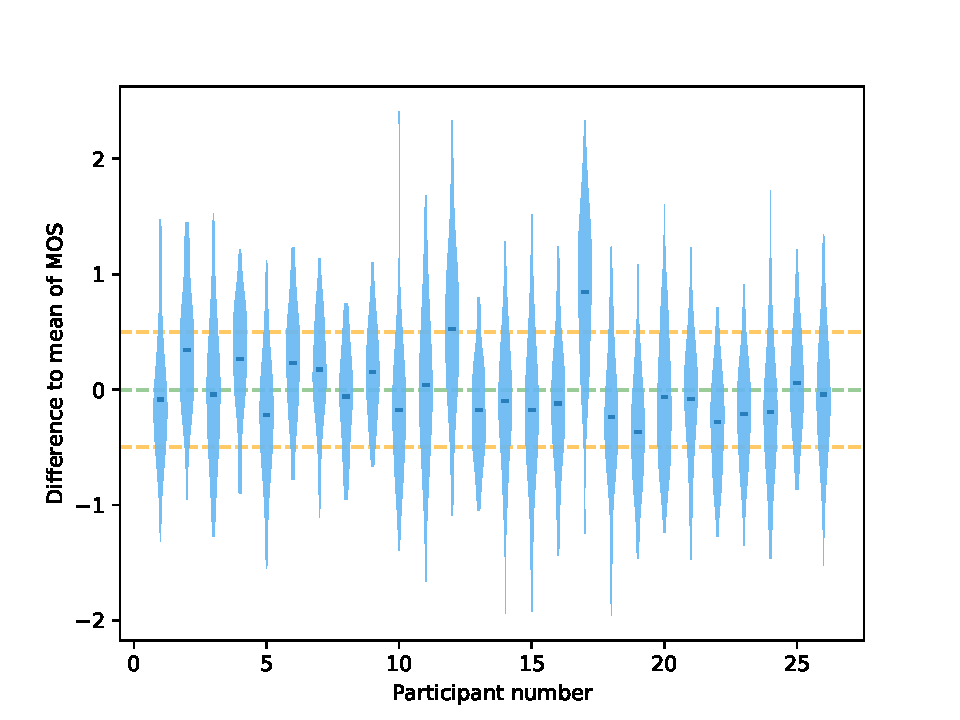
\includegraphics[width=3.5in]{participant_mos_violin}
	\caption{}
	\label{fig:result:participant_violin}
\end{figure}
\\

\textbf{Compare MOS with vmaf (correlation?)}
\begin{figure}[bht!]
	\centering
	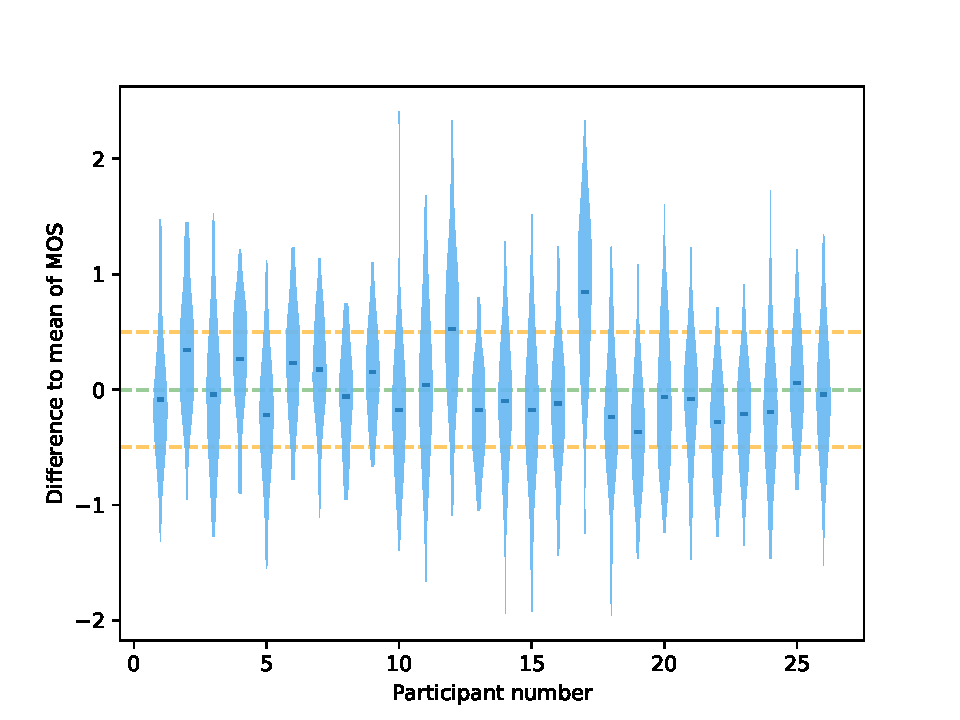
\includegraphics[width=3.5in]{participant_mos_violin}
	\caption{}
	\label{fig:result:participant_violin}
\end{figure}
\\

\textbf{Bitrate savings}
\begin{figure}[bht!]
	\centering
	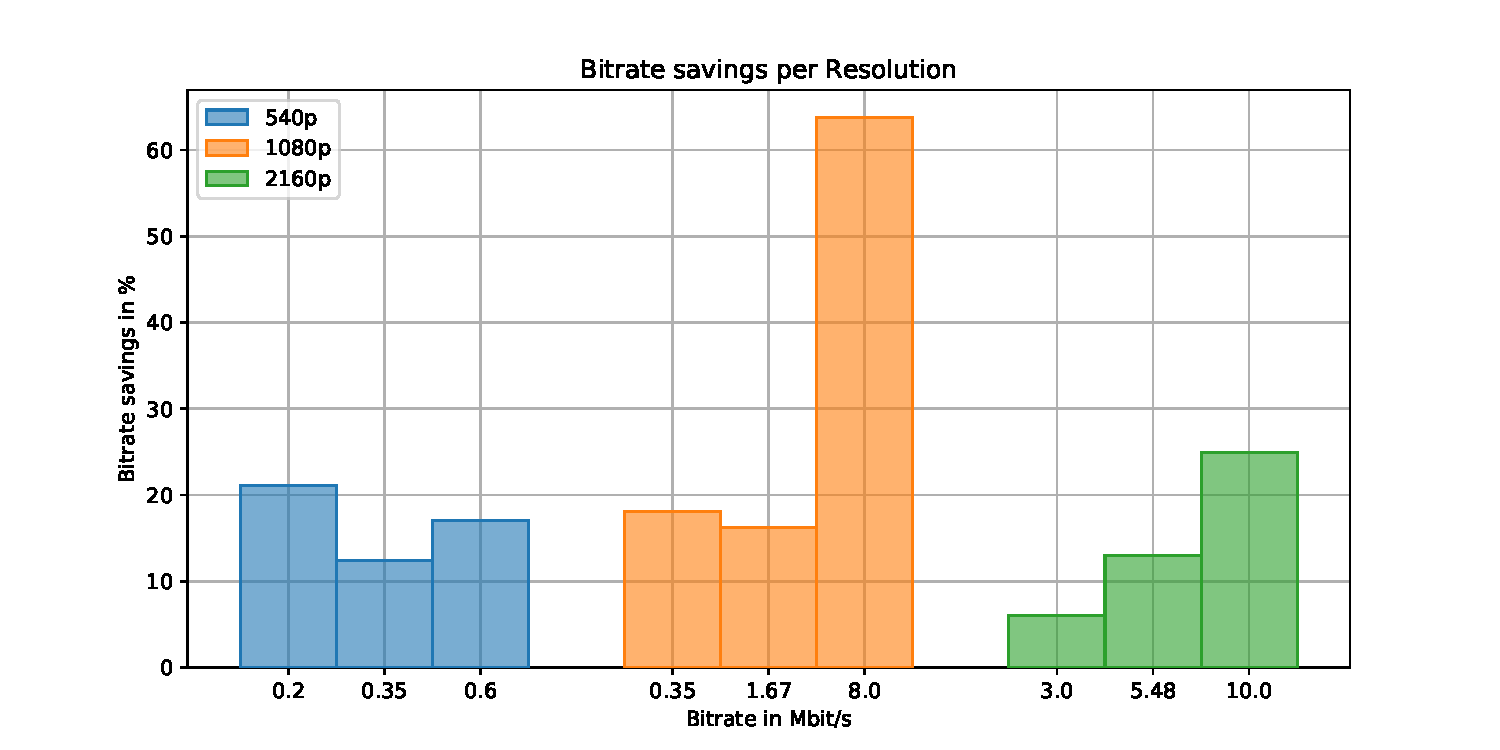
\includegraphics[width=3.5in]{bitrate_savings}
	\caption{}
	\label{fig:result:bitrate_savings}
\end{figure}
\begin{figure}[bht!]
	\centering
	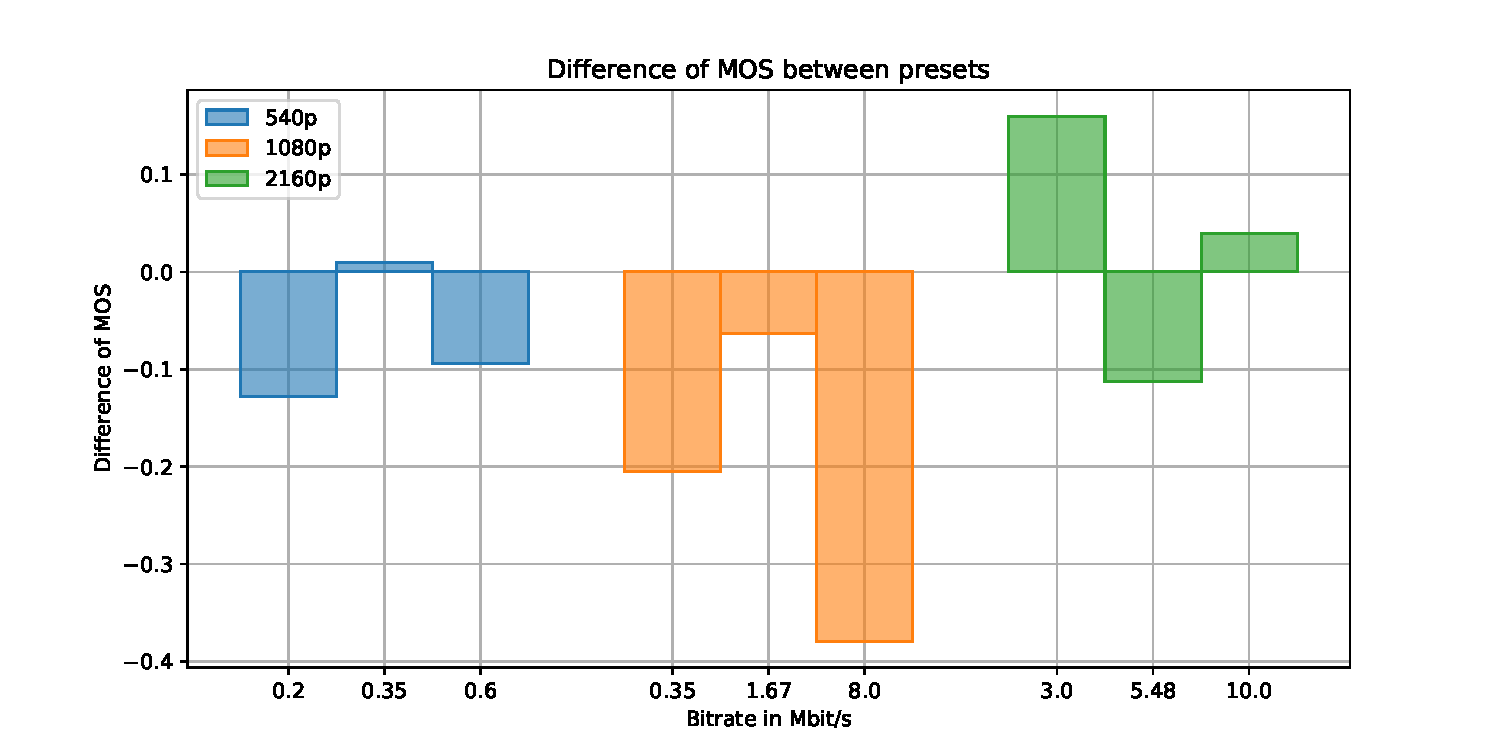
\includegraphics[width=3.5in]{quality_difference}
	\caption{}
	\label{fig:result:quality_difference}
\end{figure}